\documentclass{standalone}
\usepackage{pgfplots}
\pgfplotsset{compat=1.18}
\usetikzlibrary{external}
\tikzexternalize

\begin{document}
	
	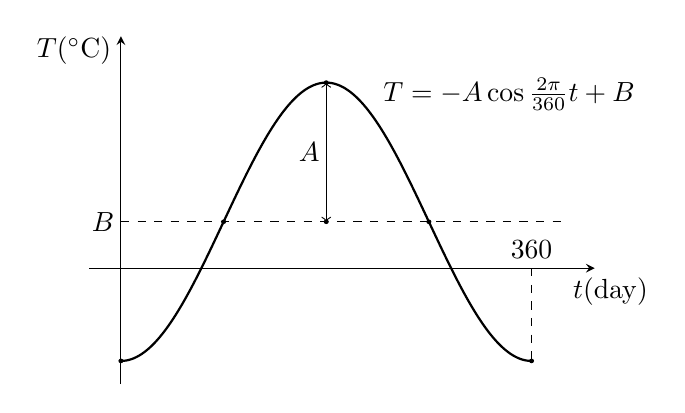
\begin{tikzpicture}
		\begin{axis}[
			xmin=-0.5, xmax=7.5,
			ymin=-2, ymax=4,
			domain=0:6.5,
			samples=1000,
			axis lines=middle,
			clip=false,			
			width=8cm,
			height=6cm,
			ticks=none
			]
			\draw[dashed] (0, 0.8) -- (7, 0.8);
			\draw[<->] (3.25, 0.8) -- (3.25, 3.2);
			\addplot [black, thick] {-2.4*cos(deg(x)*4*pi/13)+0.8};
			\draw[dashed] (6.5, 0) -- (6.5, -1.6);
			\fill[] (3.25, 0.8) circle (0.04);
			\fill (3.25, 3.2) circle (0.04);
			\fill (6.5, -1.6) circle (0.04);
			\fill (0, -1.6) circle (0.04);
			\fill (1.625, 0.8) circle (0.04);
			\fill (4.875, 0.8) circle (0.04);
			
			\node[below] at (7.75,0) {$t (\mathrm{day})$};
			\node[left] at (0,3.75) {$T (\mathrm{^\circ C}$)};
			\node[left] at (3.3, 2) {$A$};
			\node[above] at (6.5, 0) {$360$};
			\node[left] at (0.05, 0.8) {$B$};
			\node[right] at (4, 3) {$T = -A\cos{\frac{2\pi}{360} t} + B$};
		\end{axis}

	\end{tikzpicture}
	
\end{document}